\documentclass[aspectratio=169,12pt]{beamer}

\usepackage[utf8]{inputenc}
\usepackage[T1]{fontenc}
\usepackage{lmodern}
\usepackage{amsmath,amssymb}
\usepackage{bm}
\usepackage{graphicx}
\usepackage{tikz}
\usetikzlibrary{arrows.meta,positioning,shapes.geometric,fit,calc}
\usepackage{pgfplots}
\pgfplotsset{compat=1.18}
\usepackage{booktabs}
\usepackage{xcolor}
\usepackage{algorithm}
\usepackage{algpseudocode}

\usetheme{Madrid}
\usecolortheme{default}
\usefonttheme{professionalfonts}

\definecolor{mlblue}{RGB}{0,82,147}
\definecolor{mlorange}{RGB}{220,100,0}
\definecolor{mlgreen}{RGB}{0,130,70}
\definecolor{mlgray}{RGB}{80,80,80}

\setbeamercolor{structure}{fg=mlblue}
\setbeamercolor{block title}{bg=mlblue,fg=white}
\setbeamercolor{block body}{bg=mlblue!10}
\setbeamercolor{alerted text}{fg=mlorange}

\newcommand{\R}{\mathbb{R}}
\newcommand{\vect}[1]{\bm{#1}}
\newcommand{\mat}[1]{\mathbf{#1}}

\title[Redes Neuronales]{Introducción a las Redes Neuronales Artificiales}
\subtitle{De la neurona biológica al aprendizaje profundo}
\author[J. García]{Juan García}
\institute[UNAM]{Departamento de Ciencias de la Computación \\ UNAM}
\date{Abril 2026}

\begin{document}

\begin{frame}
  \titlepage
\end{frame}

\begin{frame}{Contenido}
  \tableofcontents
\end{frame}

%% ── SECCIÓN 1 ─────────────────────────────────────────────────────────────────
\section{Motivación}

\begin{frame}{¿Por qué redes neuronales?}
  \begin{columns}[T]
    \begin{column}{0.55\textwidth}
      \textbf{Problemas donde sobresalen:}
      \begin{itemize}
        \item Reconocimiento de imágenes
        \item Procesamiento de lenguaje natural
        \item Síntesis de voz y música
        \item Juegos (AlphaGo, AlphaFold)
      \end{itemize}
      \vspace{0.5em}
      \textbf{¿Qué tienen de especial?}
      \begin{itemize}
        \item Aprendizaje de representaciones jerárquicas
        \item Escalabilidad con datos y cómputo
        \item Flexibilidad arquitectónica
      \end{itemize}
    \end{column}
    \hfill
    \begin{column}{0.40\textwidth}
      \centering
      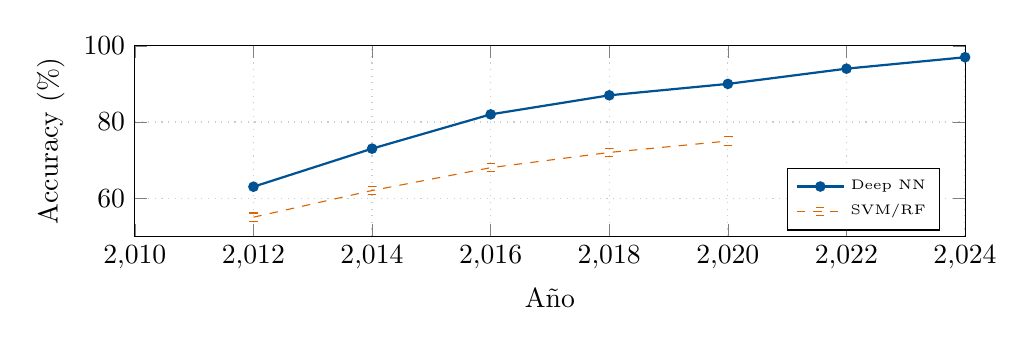
\begin{tikzpicture}
        \begin{axis}[
          width=\textwidth, height=4cm,
          xlabel={Año}, ylabel={Accuracy (\%)},
          xmin=2010, xmax=2024,
          ymin=50, ymax=100,
          grid=major, grid style={dotted,gray!40},
          legend pos=south east,
          legend style={font=\tiny},
        ]
          \addplot[mlblue,thick,mark=*,mark size=1.5]
            coordinates {(2012,63)(2014,73)(2016,82)(2018,87)(2020,90)(2022,94)(2024,97)};
          \addplot[mlorange,dashed,mark=square,mark size=1.5]
            coordinates {(2012,55)(2014,62)(2016,68)(2018,72)(2020,75)};
          \legend{Deep NN, SVM/RF}
        \end{axis}
      \end{tikzpicture}
      \tiny ImageNet Top-5 Accuracy
    \end{column}
  \end{columns}
\end{frame}

%% ── SECCIÓN 2 ─────────────────────────────────────────────────────────────────
\section{La Neurona Artificial}

\begin{frame}{Del perceptrón a la neurona moderna}
  \begin{block}{Modelo del perceptrón (Rosenblatt, 1958)}
    \begin{equation}
      y = \begin{cases} 1 & \text{si } \sum_{j} w_j x_j + b \geq 0 \\ 0 & \text{en otro caso} \end{cases}
    \end{equation}
  \end{block}
  \vspace{0.4em}
  \begin{block}{Neurona diferenciable (neurona sigmoide)}
    \begin{equation}
      y = \sigma\!\left(\sum_{j=1}^{d} w_j x_j + b\right), \quad \sigma(z) = \frac{1}{1+e^{-z}}
    \end{equation}
  \end{block}
  \vspace{0.3em}
  \centering
  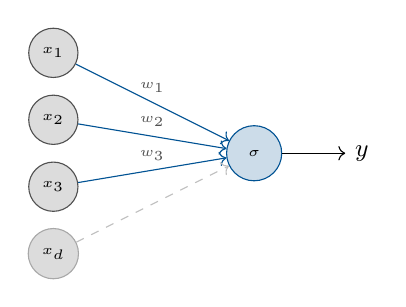
\begin{tikzpicture}[scale=0.85,
    input/.style={circle,draw=mlgray,fill=mlgray!20,minimum size=0.55cm},
    neuron/.style={circle,draw=mlblue,fill=mlblue!20,minimum size=0.7cm},
  ]
    \node[input] (x1) at (0, 1.5) {\tiny $x_1$};
    \node[input] (x2) at (0, 0.5) {\tiny $x_2$};
    \node[input] (x3) at (0,-0.5) {\tiny $x_3$};
    \node[input,draw=mlgray!50] (xd) at (0,-1.5) {\tiny $x_d$};
    \node[neuron] (n) at (3, 0) {\tiny $\sigma$};
    \node[right=0.8cm of n] (y) {\small $y$};
    \foreach \i in {1,2,3}
      \draw[->,mlblue] (x\i) -- (n) node[midway,above,font=\tiny,mlgray]{$w_\i$};
    \draw[->,gray!50,dashed] (xd) -- (n);
    \draw[->] (n) -- (y);
  \end{tikzpicture}
\end{frame}

\begin{frame}{Funciones de activación}
  \centering
  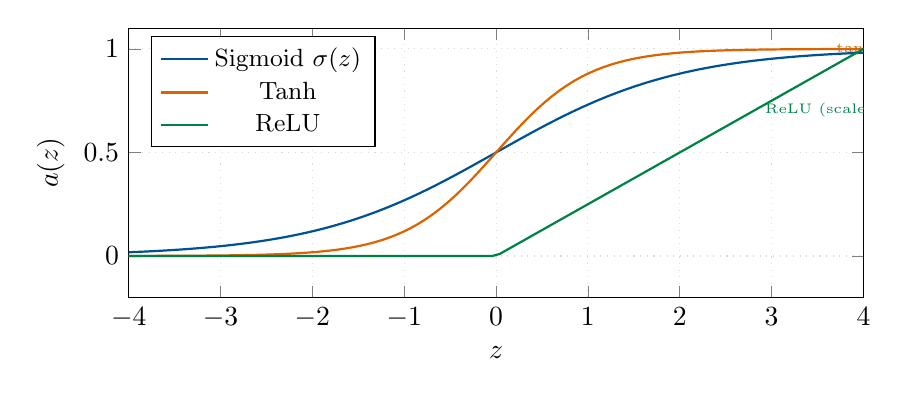
\begin{tikzpicture}
    \begin{axis}[
      width=0.9\textwidth, height=5cm,
      xlabel={$z$}, ylabel={$a(z)$},
      xmin=-4, xmax=4, ymin=-0.2, ymax=1.1,
      grid=major, grid style={dotted,gray!30},
      legend pos=north west,
      legend style={font=\small},
    ]
      \addplot[mlblue,thick,domain=-4:4,samples=100]
        {1/(1+exp(-x))} node[right,pos=1]{\tiny sigmoid};
      \addplot[mlorange,thick,domain=-4:4,samples=100]
        {tanh(x)/2+0.5} node[right,pos=0.95]{\tiny tanh (norm.)};
      \addplot[mlgreen,thick,domain=-4:4,samples=100]
        {max(0,x)/4} node[right,pos=0.85]{\tiny ReLU (scaled)};
      \legend{Sigmoid $\sigma(z)$, Tanh, ReLU}
    \end{axis}
  \end{tikzpicture}
\end{frame}

%% ── SECCIÓN 3 ─────────────────────────────────────────────────────────────────
\section{Redes Multicapa (MLP)}

\begin{frame}{Perceptrón Multicapa (MLP)}
  \begin{columns}[T]
    \begin{column}{0.45\textwidth}
      \textbf{Capas de una red feedforward:}
      \begin{enumerate}
        \item \textbf{Entrada:} $\vect{x} \in \R^{d}$
        \item \textbf{Ocultas:} transformaciones no lineales
        \item \textbf{Salida:} predicción $\hat{y}$
      \end{enumerate}
      \vspace{0.5em}
      \textbf{Forward pass (capa $l$):}
      \begin{align}
        \vect{z}^{(l)} &= \mat{W}^{(l)}\vect{a}^{(l-1)} + \vect{b}^{(l)} \\
        \vect{a}^{(l)} &= \sigma\!\left(\vect{z}^{(l)}\right)
      \end{align}
    \end{column}
    \hfill
    \begin{column}{0.50\textwidth}
      \centering
      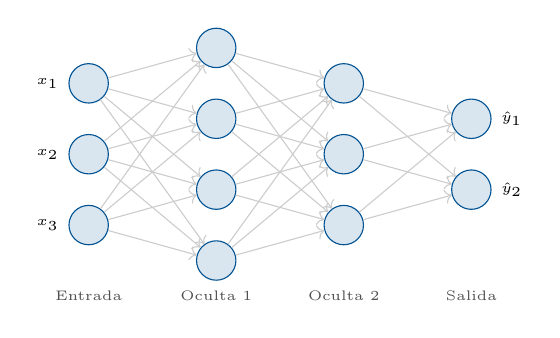
\begin{tikzpicture}[
        n/.style={circle,draw=mlblue,fill=mlblue!15,minimum size=0.5cm,inner sep=0},
        scale=0.9,
      ]
        \foreach \i/\y in {1/2, 2/1, 3/0}
          \node[n,label=left:{\tiny $x_\i$}] (i\i) at (0,\y) {};
        \foreach \i/\y in {1/2.5,2/1.5,3/0.5,4/-0.5}
          \node[n] (h1\i) at (1.8,\y) {};
        \foreach \i/\y in {1/2,2/1,3/0}
          \node[n] (h2\i) at (3.6,\y) {};
        \foreach \i/\y in {1/1.5,2/0.5}
          \node[n,label=right:{\tiny $\hat{y}_\i$}] (o\i) at (5.4,\y) {};
        \foreach \i in {1,2,3}
          \foreach \j in {1,2,3,4}
            \draw[->,gray!40,thin] (i\i) -- (h1\j);
        \foreach \i in {1,2,3,4}
          \foreach \j in {1,2,3}
            \draw[->,gray!40,thin] (h1\i) -- (h2\j);
        \foreach \i in {1,2,3}
          \foreach \j in {1,2}
            \draw[->,gray!40,thin] (h2\i) -- (o\j);
        \node[mlgray,font=\tiny] at (0,-1) {Entrada};
        \node[mlgray,font=\tiny] at (1.8,-1) {Oculta 1};
        \node[mlgray,font=\tiny] at (3.6,-1) {Oculta 2};
        \node[mlgray,font=\tiny] at (5.4,-1) {Salida};
      \end{tikzpicture}
    \end{column}
  \end{columns}
\end{frame}

%% ── SECCIÓN 4 ─────────────────────────────────────────────────────────────────
\section{Entrenamiento}

\begin{frame}{Función de pérdida y retropropagación}
  \begin{block}{Función de pérdida (clasificación)}
    \begin{equation}
      \mathcal{L}(\theta) = -\frac{1}{N}\sum_{i=1}^{N}\sum_{k=1}^{K}
      y_{ik}\log\hat{y}_{ik}
      \quad\text{(entropía cruzada)}
    \end{equation}
  \end{block}
  \vspace{0.3em}
  \begin{block}{Regla de la cadena (backpropagation)}
    \begin{equation}
      \frac{\partial \mathcal{L}}{\partial \mat{W}^{(l)}}
      = \frac{\partial \mathcal{L}}{\partial \vect{z}^{(l)}}
        \cdot \left(\vect{a}^{(l-1)}\right)^\top
      = \bm{\delta}^{(l)}\left(\vect{a}^{(l-1)}\right)^\top
    \end{equation}
  \end{block}
\end{frame}

\begin{frame}{Descenso de gradiente estocástico (SGD)}
  \begin{algorithm}[H]
    \caption{Mini-batch SGD}
    \begin{algorithmic}[1]
      \Require tasa de aprendizaje $\eta$, tamaño de batch $B$
      \State Inicializar $\theta$ (Xavier / He initialization)
      \For{cada época $e = 1, \ldots, E$}
        \For{cada mini-batch $\mathcal{B} \subset \mathcal{D}$, $|\mathcal{B}|=B$}
          \State $\hat{g} \leftarrow \frac{1}{B}\sum_{i\in\mathcal{B}}\nabla_\theta\ell(f_\theta(\vect{x}_i), y_i)$
          \State $\theta \leftarrow \theta - \eta\,\hat{g}$
        \EndFor
      \EndFor
    \end{algorithmic}
  \end{algorithm}
  \vspace{0.3em}
  \textbf{Variantes:} SGD+momentum, AdaGrad, RMSProp, \alert{Adam}
\end{frame}

%% ── SECCIÓN 5 ─────────────────────────────────────────────────────────────────
\section{Regularización}

\begin{frame}{Sobreajuste y regularización}
  \begin{columns}[T]
    \begin{column}{0.48\textwidth}
      \begin{alertblock}{Sobreajuste}
        El modelo memoriza datos de entrenamiento; falla en test.
      \end{alertblock}
      \vspace{0.4em}
      \textbf{Técnicas de regularización:}
      \begin{itemize}
        \item $L_2$: $\mathcal{L} \mathrel{+}= \frac{\lambda}{2}\norm{\theta}^2$
        \item $L_1$: $\mathcal{L} \mathrel{+}= \lambda\norm{\theta}_1$
        \item \textbf{Dropout}: apagar neuronas aleatoriamente
        \item \textbf{Data augmentation}
        \item \textbf{Early stopping}
        \item \textbf{Batch normalization}
      \end{itemize}
    \end{column}
    \hfill
    \begin{column}{0.48\textwidth}
      \centering
      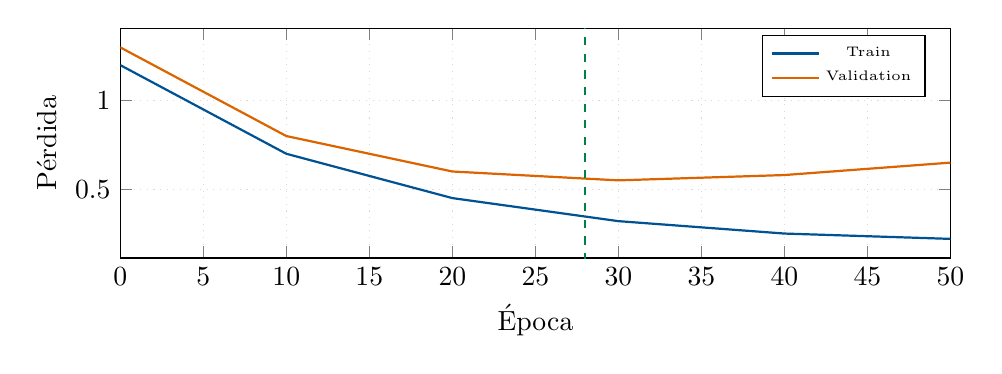
\begin{tikzpicture}
        \begin{axis}[
          width=\textwidth, height=4.5cm,
          xlabel={Época}, ylabel={Pérdida},
          xmin=0, xmax=50,
          legend pos=north east,
          legend style={font=\tiny},
          grid=major, grid style={dotted,gray!30},
        ]
          \addplot[mlblue,thick] coordinates
            {(0,1.2)(10,.7)(20,.45)(30,.32)(40,.25)(50,.22)};
          \addplot[mlorange,thick] coordinates
            {(0,1.3)(10,.8)(20,.6)(30,.55)(40,.58)(50,.65)};
          \draw[dashed,mlgreen,thick] (axis cs:28,0) -- (axis cs:28,1.5)
            node[above,font=\tiny]{early stop};
          \legend{Train, Validation}
        \end{axis}
      \end{tikzpicture}
    \end{column}
  \end{columns}
\end{frame}

%% ── SECCIÓN 6 ─────────────────────────────────────────────────────────────────
\section{Conclusiones}

\begin{frame}{Conclusiones}
  \begin{block}{Resumen}
    \begin{enumerate}
      \item Las RNA modelan funciones complejas mediante capas de neuronas no lineales
      \item El entrenamiento usa backpropagation + descenso de gradiente
      \item La regularización es clave para generalizar a datos no vistos
    \end{enumerate}
  \end{block}
  \vfill
  \begin{alertblock}{Próximos temas}
    \begin{itemize}
      \item Redes Convolucionales (CNN) para visión
      \item Redes Recurrentes (RNN, LSTM) para secuencias
      \item Transformers y mecanismo de atención
    \end{itemize}
  \end{alertblock}
\end{frame}

\begin{frame}
  \centering
  \vspace{0.8cm}
  {\Huge\bfseries\color{mlblue} ¡Gracias!}\\[1em]
  {\large Preguntas}\\[2em]
  \small \texttt{jgarcia@fciencias.unam.mx}
\end{frame}

\end{document}
